\appendix

\section*{\centering Appendix} 

%\section{Materials and Methods}\label{sect:materials_methods}
% \tobo{Why is the section not called Material and Methods?} \tsn{As far as I can tell: We should change "Methods" here and above to "Material and Methods". We refer to both, and as far as I can see, the references are to material in the section below. UPDATE: Changed all instances of "Methods" to "Material and Methods"}

 %\small

\section{Experimental design and data collection} A large total sample size of $N=870$ was chosen to get robust conclusions from the statistical analysis while giving room for high variability in behavior. In fact, we thought that there would be a minority of pairs
opting for the all-office strategy. This turned out not to be the case. Experiments on Amazon Mechanical Turk had a total of 714 participants (including dropouts, see Appendix \ref{app:mturk-walkthrough}), while the two classroom experiments at the Technical University of Denmark (DTU1 and DTU2) had a total of 106 and 50 participants, respectively\footnote{Complete anonymized data files and all code can be downloaded from \url{https://github.com/gavstrik/Paper_canteen_dilemma}.}

The average payout to MTurk workers was \$4.17 (including a general participation fee of \$2). After accepting our task and providing informed consent, participants from MTurk were put in a ’waiting room’ until they were paired up with another participant. After an instructions page, detailing the rules of the game, participants were given an arrival time $t \in \{8{:}00, 8{:}10, 8{:}20, 8{:}30, 8{:}40, 8{:}50, 9{:}00,9{:}10\}$ and asked to make a decision \modified{between} going to the canteen or to the office. Next, participants were asked to estimate how certain they were that their `colleague' made the same choice as them, ranging from `very uncertain' over `slightly certain', `somewhat certain' and `quite certain' to `very certain', which were translated  into numerical values, $e_i$, used in the payoff calculations (see below). A results page was shown between each round, showing the results of the previous rounds, including arrival times for both players, their choices, their own certainty estimates and resulting payoffs. After 30 seconds, the game would automatically proceed to the next round. After the last round, we asked all participants a few final questions about their strategy and their understanding of the game. The experiments were implemented using oTree 2.1.35~\cite{ChenSchongerWickens16}.

The two classroom experiments, DTU1 and DTU2, differed from the MTurk experiment in a few aspects: 1) the maximum number of rounds played was increased from 10 to 30; 2) the initial bonus given each participant was increased accordingly from \$10 to \$30; 3) three additional questions were asked in order to elicit more explicitly some of the implicit assumptions and explicit behaviours by the students; 4) participants were told that they would not receive any monetary rewards, but that they should try to do their best. DTU1 received prizes. Screenshots, additional questions, experimental settings, and a detailed walk-through can be found in Appendix \ref{app:materials-methods-further}.

\subsection{Mixed effect logistic regression} \label{appendix:logistic} 
The experimental results were also analyzed using a generalized mixed-effects logistic regression model in R (\emph{glmer}), with the arrival time $t$ and experimental condition $exp$ (MTurk, DTU1, DTU2) as fixed effects including interactions and random effects for each pair of players, because we expect pairs to behave differently, depending on which levels of shared knowledge they individually take into account in their reasoning and collectively try to agree upon. Exploratory analysis including the round number as an additional fixed effect did not show any significant contributions, meaning that players did not significantly change their strategy during the game. %The model was specified as $\mu_i = \alpha _{i} + \beta _{i}t + W_{ij}$, with $\mu_i$ being the log-odds $\mu_i= \log (p_i/(1-p_i))$ and $W_{ij} is the pair-specific random effect, i.e., it's the deviation of the j-th pairs’s score from the average for the i-th experiment. $i=1,2,3$ denoting the MTurk, DTU1 and DTU2 experiments, respectively, allowing for differing slopes and intercepts. 

\begin{figure} % [!b]
	\centering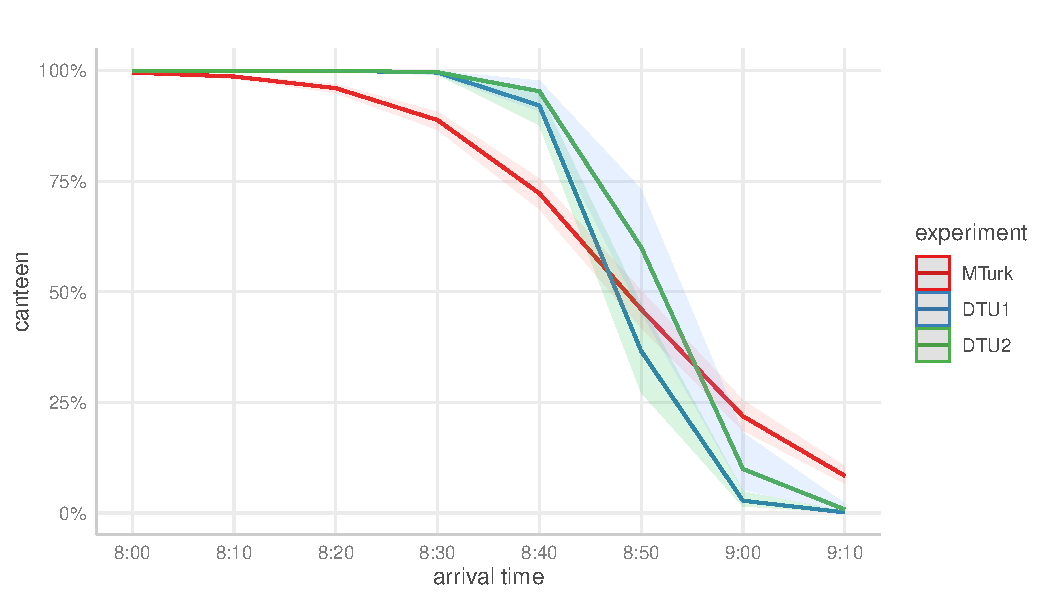
\includegraphics[width=0.8\linewidth]{fig1_regression}
	\caption{Percentage of canteen choices as a function of arrival times. The colored lines are logistic regression lines from a mixed-effects model with 95\% confidence intervals shown as translucent bands. Fitted parameters show significant differences in the slope and intercept between MTurk and DTU experiments ($p < .0001$).}
	\label{fig:mx}
\end{figure}

Using a generalized linear mixed-effects model with the arrival time and the three experimental conditions as fixed effects and with player-pairs as random effects, we obtain a logistic regression fit in Fig.~\ref{fig:mx}, showing the probability of players choosing the canteen as a function of their arrival time.Results from the mixed-effects  model are almost indistinguishable from the simple logit model without random effects used in Fig.~\ref{fig:1} The steepest slope occurs at $p(t) = 1/2 = -\alpha/\beta$, which for the MTurk and DTU1 experiments is $t=8{:}48$ and for DTU2 is $t=8{:}52$. The regression line in Fig.~\ref{fig:indistinguish} is obtained by combining observations from all three experiments and using a simple logistic regression model without random effects. The high number of observations imply small confidence bands. Hence, conclusions from the models can be viewed as robust. Code and data are available on github (\url{https://github.com/gavstrik/Paper_canteen_dilemma}).


\section{Payoffs and Penalties} \label{appendix:payoffs}
 All MTurk players finishing the game were paid a participation fee of \$2. In addition, a bonus could be earned if players did well. Before the game started, the bonus was set to \$10 for all participants. After each round, the bonus was reduced by a personal penalty, depending on the two players' choices. Penalties are calculated using a logarithmic scoring rule and by ordering them to be minimized by successful coordinations into the canteen. Penalties are maximized by any type of miscoordination or forbidden choice (i.e.\ going to the canteen at 9:00 or later). Office coordinations are designed to have larger penalties than canteen coordinations, but smaller penalties than miscoordinations in order to make sure that coordination remains the main objective of the game. Penalties are defined as negative utility values in the following way. First, we define the chosen action $a_i$ by player $i$, $i=1,2$, to take binary values encoding the canteen option ($a_i=0$) and the office option ($a_i=1$), and define their respective certainty estimates $e_i \in \{0.5, 0.625, 0.75, 0.875, 0.99\}$. We can then express the utility $u$ received by player $1$ as $u(e_1, a_1, a_2) = (1-|a_1-a_2| + a_1a_2)ln(e_1) + 2|a_1-a_2|ln(1-e_1)$, and symmetric for player 2. If any of the players choose the canteen at 9:00 or after, the utility becomes $u(e_1,a_1,a_2) = 2ln(1-e_1)$ for player 1 (and symmetric for player 2), corresponding to a miscoordination. As an example, imagine player 1 arrives at $8{:}40$ and choses the canteen, $a_1=0$. She estimates the probability that her colleague also will to go to the canteen to ``somewhat certain'', $e_1=0.75$. If her colleague indeed chooses the canteen, $a_2=0$, her utility will be $u(e_1,a_1,a_2) = ln(e_1) = -0.29$, but if her prediction proves false and her colleague chooses the office instead, her utility will be $u(e_1,a_1,a_2) = 2ln(1-e_1)=-2.77$. If she goes to the office just like her colleague, her utility is $u(e_1,a_1,a_2) = 2ln(e_1)=-0.58$. It should be noted that the logarithmic scoring rule used here is strictly proper. It is therefore not surprising that we find a good match between estimates and actual choices at arrival times different from those that are prone to miscoordinations, as seen in Fig.~\ref{fig:certain}, indicating that loss minimization remained a central concern and that participants made their choices and estimates as honestly as possible \cite{good1992rational, seidenfeld1985calibration, palfrey2009eliciting}.

\section{Formal Analysis} \label{appendix:formal}
We now give a detailed formal analysis of the game. We want to keep things as general as possible, so we don't assume a particular payoff structure, but any payoff structure satisfying certain constraints, and we want to consider arbitrary strategies, also mixed ones. This makes the analysis a bit non-trivial, although the underlying intuitions are rather straightforward. We of course haven't expected our human subjects to have made a deep analysis corresponding to the one below before starting to play the game. That should also not be necessary: The crucial aspect is to realize that there is no time point at which it is safe to go to the canteen (and hence avoid the high penalty), and this only requires to reason that 8{:}50 is not safe, and that then also 8{:}40 is not safe, and that then also... etc. What we do below is just to verify in a generalised setting that this reasoning is indeed formally correct and game theoretically valid and acting according to it leads to the highest expected payoff.  

The game can be represented as a game with three players, \emph{nature}, \emph{player 1} and \emph{player 2}. Nature is the player that initially decides the arrival times of player 1 and 2. Then player 1 and 2 are each informed of their own arrival time, and each have to choose among two actions: $o$ for going to the office and $c$ for going to the canteen. Based on the choice of actions by all three agents, player 1 and 2 receive a payoff. The payoff for player 1 is always equal to the payoff for player 2 (common payoff game). We  disregard the certainty estimates for now. The action choice of nature can be represented as an \emph{arrival pair} ${\bf t} = (t_1,t_2)$ consisting of the arrival time $t_1$ for player 1 and $t_2$ for player 2. Any arrival pair $\bf t$ has to satisfy that  $| t_1 - t_2 | = 0{:}10$. In our specific version of the game, we additionally have the restriction that \modified{$8{:}00 \leq t_i \leq 9{:}10$} for $i = 1,2$. The analysis of optimal strategies however doesn't depend on the exact arrival times available, so we will make things a bit more general and only assume that there is an earliest arrival time $\tmin$ and a latest arrival time $\tmax$, and that $\tmin \leq 8{:}50$ and $\tmax \geq 9{:}00$. Since we are counting in tens of minutes, by slight abuse of language we will call an arrival time \emph{even} if it is of the form $9{:}00+0{:}20x$ for some integer $x$, and \emph{odd} if it is of the form $9{:}00+0{:}10+0{:}20x$. The game then naturally splits into two disjoint subgames: in one of these subgames, player 1 always arrives at an odd time, and player 2 at an even time; 
%arrives at a time $\tmin+20x$ for some $x \geq 0$ and player 2 arrives at a time $\tmin+20x+10y$ for some $y \in \{-1,1\}$. 
 in the other subgame, the arrival time of the two players are reversed. The two subgames are disjoint in the sense that it is always common knowledge among the players which of the two arrived at an even time. We can hence restrict focus to one of the two subgames. We will pick the subgame where player 1 arrives at an odd time. To simplify further, we can without loss of generality assume that both $\tmin$ and $\tmax$ are also odd times. All reasoning performed in the following generalises immediately to the other subgame and to other values of $\tmin$ and $\tmax$. 
 
We let $T$ denote the set of arrival times and $\bf T$ the set of arrival pairs.  
The game starts by nature choosing an element $\mathbf{t} \in \bf T$. Nature is not a strategic player, so we assume that $\bf t$ is chosen uniformly at random, which is exactly how $\bf t$ is chosen in our experiments. The participants do not know that the arrival times are chosen uniformly at random, as this is left implicit in the description of the game. The following analysis of optimal strategies in the game could potentially change if arrival times were chosen according to a highly skewed probability distribution.

When nature has chosen its action ${\bf t} \in \bf T$ and player 1 and 2 have chosen their actions $a_1$ and $a_2$, player 1 and 2 receive their payoff, which we denote $u_\mathbf{t}(a_1,a_2)$ (the utility resulting from player 1 choosing $a_1$ and player 2 choosing $a_2$ given that nature played $\bf t$). We don't need to make any assumptions regarding the exact utility values (payoff values), except that successful coordination into the canteen before $9{:}00$, denoted $u_\mathit{c}$, is always better than successful coordination into the offices, denoted $u_\mathit{o}$, which again is always better than being miscoordinated, denoted $u_\mathit{m}$. Hence we suppose given fixed utility values $u_\mathit{c} > u_\mathit{o} > u_\mathit{m}$ such that for all ${\bf t} = (t_1,t_2) \in {\bf T}$,  $u_{\bf t}(o,o) = u_\mathit{o}$, $u_{\bf t}(o,c) = u_{\bf t}(c,o) = u_\mathit{m}$ and 
\[
u_{\bf t}(c,c) = 
\begin{cases}
   u_\mathit{c} &\text{if $t_1,t_2 < 9{:}00$} \\
   u_\mathit{m} &\text{otherwise}
\end{cases}
\]
 % such that 
%Hence, we put the following constraints on the utility function, for all  ${\bf t} = (t_1,t_2) \in \bf T$,
%\begin{enumerate}
%   \item[(U1)] $u_\mathbf{t}(o, o) > u_\mathbf{t}(c,o) = u_\mathbf{t}(o,c)$.
%   \item[(U2)] If $t_1,t_2 < 9{:}00$ then $u_\mathbf{t}(c,c) > u_\mathbf{t}(o, o)$ else $u_\mathbf{t}(c,c) = u_\mathbf{t}(c,o) = u_\mathbf{t}(o,c)$.
 %\end{enumerate}

A \emph{strategy} % for player $i$, $i =1,2$,
 is a mapping from arrival times to actions, that is, 
 %a probability distribution over actions, that is,
   a mapping $s: T \to \{c,o\}$. 
   %    \Pi(\{c,o\})$ where $\Pi(X)$ denotes the set of probability distributions over $X$~\cite{shoham2008multiagent}. 
%   Hence, for each $t \in T$,
   % and each $x \in \{c,o\}$,  $s(t)(x)$ denotes the probability of choosing $x$ at arrival time $t$. 
  % $s(t)$ is the chosen action at time $t$.
 Normally one would define two strategies, one for each player. That is however not necessary in our game. By assumption, player 1 can only observe odd arrival times, so if $t$ is odd, $s(t)$ denotes the strategic choice of player 1 at $t$, otherwise of player 2 at $t$. In this way $s$ encodes a \emph{strategy profile} (a strategy for each player). Since each player only observe their own arrival time, their strategic choice can only depend on their observed arrival time, which is why $s$ is a mapping from $T$ rather than from $\bf T$.   
%A strategy for $i$ simply determines which action $i$ will choose given the arrival pair. 
%Each agent only observes her own arrival time, that is, any two arrival pairs $\mathbf{t}$ and $\mathbf{t}'$ with $t_i = t'_i$ will be indistinguishable to player $i$, $i=1,2$. This immediately leads to the following formal definition of the indistinguishability relation $\sim_i$ for player $i$: $\mathbf{t} \sim_i \mathbf{t}'$ iff $t_i = t'_i$. We need to require the strategy of each player to be \emph{uniform}, that is, any two arrival pairs that are indistinguishable by that player should be mapped to the same action: if $\mathbf{t} \sim_i \mathbf{t'}$ then $s_i(\mathbf{t}) = s_i(\mathbf{t'})$. Due to the uniformity condition, we can allow ourselves to overload the meaning of the symbol $s_i$ and write $s_i(t_i)$ as an abbreviation of $s_i(t_1,t_2)$ for $i=1,2$. 

Note that the defined strategies are memoryless (Markov strategies), that is, a player's choice only depends on the observed arrival time in the current round, not the history of arrival times and chosen actions in earlier rounds. Human players playing the game should not be expected to necessarily play memoryless strategies, as they might seek to adapt to the observed strategy of the other player. However, since it is a repeated game (every round is a new instance of the same game), perfectly rational players playing the game for a sufficient number of rounds should converge to an optimal memoryless strategy. We will leave further discussion of history-dependent strategies and focus on the optimal memoryless strategies in the following.



%Given strategies $s_1$ and $s_2$, the pair ${\bf s} = (s_1,s_2)$ is called a \emph{strategy profile}. Given an arrival pair ${\bf t} = (t_1,t_2)$, we use $\mathbf{s}(\mathbf{t})$ as a shorthand for $(s_1(t_1), s_2(t_2))$. Hence $\mathbf{s}(\mathbf{t})$ denotes the probability distribution over choices made by players 1 and 2 when their strategies are given by $\mathbf{s}$ and their arrival times are given by $\mathbf{t}$.
%We know that player 1 always arrives at odd times, so we can take ${\bf s}(t)$ to denote $s_1(t)$ when $t$ is odd and $s_2(t)$ when $t$ is even. So ${\bf s}(t)$ is the probability distribution of choices when observing $t$ by the player who observes it. 

The payoff of a strategy $s$ at an arrival pair $(t_1,t_2)$ is then defined as $u_{(t_1,t_2)}(s) = u_{(t_1,t_2)} (s(t_1),s(t_2))$.  
% follows~\cite{shoham2008multiagent}:
%\[
%u_{(t_1,t_2)}(s) := 
%\sum_{(x,y) \in \{o,c\}^2} s(t_1)(x) \cdot s(t_2)(y) \cdot u_{(t_1,t_2)}(x,y) 
%\]
%In words: We take the weighted sum of the possible utilities received at $(t_1,t_2)$, with the weight of each utility being the probability of receiving this utility---where we note that the probability that player 1 chooses $x$ and player 2 chooses $y$ at $(t_1,t_2)$ is expressed by $s(t_1)(x) \cdot s(t_2)(y)$. 
%We will use $u_\mathbf{t}(\mathbf{s})$ as an abbreviation of $u_\mathbf{t}(\mathbf{s}(\mathbf{t}))$, i.e., $u_\mathbf{t}(\mathbf{s})$ is the expected utility received by player 1 and 2 when they play by strategy profile $\mathbf{s}$ in the game with arrival pair $\mathbf{t}$. 
The \emph{expected utility} $EU(s)$ of a strategy $s$ is the average of the payoffs~\cite{shoham2008multiagent}:
\[
 EU(s) = \frac{1}{|  {\bf T} |} \sum_{{\bf t} \in \bf T} u_\mathbf{t}(s). %  \cdot P({\bf t}).
\]
Note again that player 1 and 2 get the same payoff (common-payoff game), so there is only one expected utility value to be computed. A strategy $s'$ \emph{Pareto dominates} another strategy $s$ if $EU(s') > EU(s)$ \cite{shoham2008multiagent}. \modified{Since both players receive the same payoff, this coincides with the standard notion, under which $s'$ is at least as good as $s$ for every player and strictly better for at least one.}
A strategy is \emph{Pareto optimal} if there does not exist another strategy dominating it. %A strategy profile ${\bf s}'$ \emph{weakly Pareto dominates} another strategy profile $\bf s$ if $EU({\bf s}') \geq EU({\bf s})$. 
The game is cooperative (between player 1 and 2), so both players should seek to play a Pareto optimal strategy. Also, since it is a common-payoff game, all Pareto optimal strategies have the same expected utility~\cite{shoham2008multiagent}. 

Note also that our strategies are pure. To make things as general as possible, one would normally also consider mixed strategies, i.e., probability distributions over strategies (or, equivalently, mappings of arrival times into probability distributions over actions).  However, that is not necessary here as our game is a common payoff game. As explained in~\cite{leyton2022essentials}, common payoff games always have at least one pure Pareto optimal strategy. Furthermore, any Pareto optimal mixed strategy will be a combination of pure Pareto optimal strategies. 
%a mixed strategy will be Pareto optimal if and only if it is a combination of pure Pareto optimal strategies. The 'if' direction of this statement is trivial, since we already mentioned that all Pareto optimal strategies have the same expected utility. For the 'only if' direction, note that if a mixed strategy gives a positive probability to choosing some particular pure strategy, then that pure strategy must have maximal expected utility among the choices given positive probability, since @@@ 
%all mixed Pareto optimal strategies will be combinations of pure Pareto optimal strategies. 
To see the latter, suppose, for $i=1,2$, that player $i$ has a mixed strategy $m_i \in \Pi(S_i)$, where $S_i$ is the set of possible pure strategies of player $i$, and $\Pi(X)$ denotes the set of probability distributions over $X$~\cite{shoham2008multiagent} (in our particular game, $S_1$ would assign choices to only the odd arrival times, and $S_2$ to the even). Suppose further that the strategy profile $(m_1,m_2)$ is Pareto optimal. Let $S'_i \subseteq S_i$ denote the subset of strategies that are assigned positive probability in $m_i$. 
%A pure strategy profile $(s_1,s_2) \in S_1 \times S_2$ is said to have support in $(m_1,m_2)$ if $m_1(s_1) > 0$ and $m_2(s_2) > 0$ (the pure strategy profile is chosen with positive probability). 
Each pure strategy profile $(s_1,s_2) \in S'_1 \times S'_2$ has an expected utility. Consider a pure strategy profile $(s_1,s_2) \in S'_1 \times S'_2$ that has maximal expected utility among all policy profiles in $S'_1 \times S'_2$. Suppose there exists another strategy profile $(s'_1,s'_2) \in S'_1 \times S'_2$ with strictly lower expected utility. If that's the case, then the pure strategy profile $(s_1,s_2)$ has higher expected utility than the mixed strategy profile $(m_1,m_2)$, which contradicts the assumption. Hence all strategy profiles $(s'_1,s'_2) \in S'_1 \times S'_2$ must have the same expected utility, hence all be pure Pareto optimal strategies. This means that we can focus on finding pure Pareto optimal strategies, since any potential Pareto optimal mixed strategies will be a combination of such Pareto optimal pure strategies.   


%Define subsets of arrival pairs $T_1, T_2 \subseteq T$ by:
%\[
%  \begin{array}{l}
%  T_1 = \{ (8{:}10 + 20x, 8{:}20 + 20y) \in T \mid  y \leq x \leq y+1 \} \\
%  T_2 = \{ (8{:}20 + 20y, 8{:}10 + 20x) \in T \mid  y \leq x \leq y+1 \}
 % \end{array}
%\]
%Note that $T_1$ and $T_2$ are disjoint and that $T = T_1 \cup T_2$. We hence get, for any strategy profile $\bf s$,
%\begin{equation}\label{equation:eu-split1}
% EU({\bf s}) = \frac{1}{| T |} \sum_{{\bf t} \in T} u_\mathbf{t}(\mathbf{s}) = \frac{1}{|T|} \sum_{i \in \{1,2\} } \sum_{{\bf t} \in T_i} u_\mathbf{t}(\mathbf{s})
%\end{equation}
%Given a strategy profile $\mathbf{s}$, we let $\mathbf{s} \upharpoonright T_i$ be the restriction of $\mathbf{s}$ to $T_i$, that is, $\mathbf{s} \upharpoonright T_i$ is as $\mathbf{s}$ except it is only defined on the arrival pairs in $T_i$. So $\mathbf{s} \upharpoonright T_i$ is the strategy profile for the subgame in which only the arrival pairs in $T_i$ can be chosen. We can now rewrite formula (\ref{equation:eu-split1}) as
%\begin{equation}\label{equation:eu-split2}
% EU({\bf s}) = \frac{1}{| T |} \sum_{{\bf t} \in T} u_\mathbf{t}(\mathbf{s}) = \frac{1}{|T|}
%\sum_{i \in \{1,2\}}
%  \sum_{{\bf t} \in T_i} u_\mathbf{t}(\mathbf{s}  \upharpoonright T_i)
%\end{equation}
%Note that there exists no $\mathbf{t} \in T_1$, $\mathbf{t}' \in T_2$ and $i\in \{1,2\}$ such that $\mathbf{t} \sim_i \mathbf{t'}$. Hence the strategy profile $\mathbf{s} \upharpoonright T_1$ can be chosen completely independently of the strategy profile $\mathbf{s} \upharpoonright T_2$. Using formula (\ref{equation:eu-split2}) it then follows that a strategy profile $\mathbf{s}$ is Pareto optimal in the full game if and only if each of the strategy profiles $\mathbf{s} \upharpoonright T_1$ and $\mathbf{s} \upharpoonright T_2$ are Pareto optimal on the subgames with arrival pairs only in $T_1$ and $T_2$, respectively. When looking for Pareto optimal strategy profiles in the game, we can hence look for Pareto optimal strategy profiles on each of the two subgames independently (essentially the game consists of two disjoint subgames). Note also that the two games are completely symmetric, since $(t_1,t_2) \in T_1$ if and only if $(t_2,t_1) \in T_2$. Hence the two subgames necessarily have the exactly the same strategy profiles up to symmetry (swapping the roles of player 1 and 2). It is hence sufficient to only investigate Pareto optimal strategies for one of these subgames, say the subgame with arrival pairs in $T_1$.
We will now try to determine the possible candidates for being Pareto optimal strategies. %profiles. %We do this by iteratively removing strategy profiles that are not Pareto optimal.
\begin{lemma}\label{lemma:no-canteen-at-nine}
%Going to the canteen at $9{:}00$ or after can never be part of a Pareto optimal strategy. More precisely: 
%No strategy $s$ with $s(t)(c) > 0$ for some %$i \in \{1,2\}$ and
%$t \geq 9{:}00$  can be Pareto optimal.
If a strategy $s$ is Pareto optimal then $s(t) =o$ for all $t \geq 9{:}00$.
\end{lemma}
\begin{proof}
We prove the contrapositive. Consider a strategy $s$ with $s(t) = c$ for some $t \geq 9{:}00$. We can assume $t$ to be odd, the other case being proved similarly. This implies $t \geq 9{:}10$.
% $i\in \{1,2\}$ and
%some ${\bf t} \in T$ with $t_{i} \geq 9{:}00$. 
%We only consider the case of $i=1$, the case of $i=2$ being proved similarly. Then we have $s_1(t_1)(c) > 0$ and $t_1 = 9{:}10+20x$ for some $x$ (recall that we have restricted attention to the subgame in which player 1 arrives at an odd time). 
Now define a strategy $s'$ which is identical to $s$ except $s'(t') = o$ for all $t' \geq 9{:}00$ (meaning that for arrival times at $9{:}00$ or after, both agents go to the office).  We want to show that $s'$ Pareto dominates $s$, implying that $s$ is not Pareto optimal. First note that
%\[
%  \begin{array}{rll}
 $u_{(t,t+0{:}10)}(s') = u_o$
 by definition of $s'$.
 %  &\text{def.\ of $\mathbf{s'}$} \\
%   	&> u_{(9{:}10+20x,9{:}00+20x)}(c,\cdot) &\text{by constraint U2} \\
%	&= u_{(9{:}10+20x,9{:}00+20x)}({\bf s}), \\ 
%  \end{array}
%\]
For this arrival pair, it is impossible to receive the utility $u_c$, so $u_o$ is the highest possible payoff for this arrival pair. 
%By constraint U1 and U2, the $(o,o)$ choice has a strictly better payoff than any other choice for this arrival pair. 
Hence any strategy not specifying $(o,o)$ at this arrival pair 
%Hence any strategy that doesn't unconditionally specify $(o,o)$ at this arrival pair 
will have a strictly lower (expected) payoff. Now note that since $s(t) = c$, then $s$ does \emph{not} specify $(o,o)$ at $(t,t+0{:}10)$, and hence we get 
%Hence, in particular, the strategy profile $\mathbf{s}$ that has ${\bf s}(9{:}10+20x)(c) > 0$ will have strictly lower payoff, so 
$u_{(t,t+0{:}10)}(s') > u_{(t,t+0{:}10)}(s)$. %where the last equality follows from $s_1(9{:}10+20x) = s_1(t_1) =  c$. 
This proves the existence of an arrival pair for which $s'$ has a strictly higher utility than $s$. To prove $EU(s') > EU(s)$, we hence only need to prove that $u_\mathbf{t'}(s') \geq u_\mathbf{t'}(s)$ for all $\mathbf{t'} = (t'_1,t'_2) \in \bf T$. When $t'_1,t'_2 < 9{:}00$ this is trivial, as we then have $s'(t'_i) = s(t'_i)$ by definition of $s'$. When $t'_j \geq 9{:}00$ for some $j$, $s'(t'_j) = o$ by definition.
% of $s'$ necessarily assign the same or higher probability to $o$ than $s$. 
%Note that $u_{\bf t'}(s)$ is either $u_o$ or $u_m$. 
If $u_{\bf t'}(s) = u_m$, we immediately get $u_{\bf t'}(s') \geq u_{\bf t'}(s)$, since $u_m$ is the lowest payoff. If $u_{\bf t'}(s) = u_o$ then also $u_{\bf t'}(s') = u_o$, since $s'$ has an $o$ in all the places where $s$ has. 
% In $s'$, we have potentially replaced some $c$ choices by $o$ choices, but never the other way around, so $u_{\bf t'}(s')$ can never be  
%This means that the probability of the $(o,o)$ choice will either increase or stay unchanged ($s'$ never gives higher probability to choosing $c$ than $s$ does), and hence, again by U1 and U2, $u_\mathbf{t'}(s') \geq u_\mathbf{t'}(s)$.
\end{proof}

\begin{lemma}\label{lemma:no-c-after-o}
Let $s$ be a Pareto optimal strategy. For all arrival times $t$, if $s(t) = o$ then $s(t+0{:}10) = o$.
%If a Pareto optimal strategy $s$ has $s(t)(o) > 0$ for some $t$, then $s(t+10)(o) < \frac12$.
%Assume $s(t)(o) > 0$ and $s(t+10)(c) \geq \frac{1}{2}$ for some strategy $s$ and arrival time $t$. Then $s$ is not Pareto optimal.
\end{lemma}
\begin{proof}
We prove the contrapositive.
Suppose $s$ is a strategy with $s(t) = o$ and $s(t+0{:}10) = c$ for some $t$. We need to prove that then $s$ is not Pareto optimal, i.e., we need to find a strategy $s'$ that  Pareto dominates $s$. %We only consider the case $i=1$, the case of $i=2$ being symmetric. 
%Then we have $s_1(t)(o) >0$ and $s_2(t+10)(c) \geq \frac{1}{2}$.  
If $s(t') = c$ for some $t' \geq 9{:}00$, the existence of a strategy dominating $s$ follows
immediately from Lemma~\ref{lemma:no-canteen-at-nine}. We can hence in the following assume that $s(t') = o$ for all $t' \geq 9{:}00$.  Since $s(t+0{:}10) = c$, we can thus also conclude that $t + 0{:}10 < 9{:}00$.
Now define $s'$ to be identical to $s$ except that we let $s'(t') = c$ for all $t' \leq t$.
%\[
%  \begin{array}{ll}
%    s'_1(t-20x)(c) = 1 &\text{for } x \geq 0 \\
%    s'_2(t-10-20y)(c) = 1 &\text{for } y \geq 0,
%  \end{array}
%\]
%recalling that we are only considering arrival pairs in $T$. 
We want to show that $EU(s') > EU(s)$. First consider the arrival pair $\mathbf{t} = (t,t+0{:}10)$. We immediately get $u_{\bf t}(s') = u_c > u_m = u_{\bf t}(s)$.
%Then, by definition of expected payoff, $u_{\bf t}(s) = p q u_o  + (p(1-q) + (1-p)q) u_m + (1-p)(1-q)u_c$. In $s'$, we have the same but with $p=0$, so $u_{\bf t}(s') =  q u_m + (1-q)u_c$. We then get $u_{\bf t}(s') - u_{\bf t}(s) = p(2q-1) u_m + p(1-q) u_c - pq u_o = p(1-q) u_c - p(1-2q) u_m - pq u_o$. Since $p>0$, this is positive iff $(1-q) u_c - (1-2q) u_m - q u_o$ is. Since $q \leq \frac12$, we have $1-2q \geq 0$. Since $u_o > u_m$, we then get  $(1-q) u_c - (1-2q) u_m - q u_o \geq (1-q) u_c - (1-2q) u_o - q u_o = (1-q) (u_c - u_o)$. Since $q \leq \frac12$ and $u_c > u_o$, this expression is positive, and hence 
%0.9 uc + 0.8 u_m - 0.9u_o$u_{\bf t}(s') - u_{\bf t}(s) >0 $, as wanted. 
To prove $EU(s') > EU(s)$, it hence now only remains to prove that $u_{\bf t'}(s') \geq u_{\bf t'}(s)$ for all $\mathbf{t'} = (t'_1,t'_2) \in \bf T$. The only non-trivial case is when $t'_i \leq t$ for some $i$ 
%either $t'_1 = t - 20x$ for some $x \geq 0$ or $t'_2 = t - 10 - 20y$ for some $y \geq 0$ 
(in all other cases, $s'(\bf t') = s(\bf t')$). 
If $t'_i \leq t$ then either we also have $t'_{3-i} \leq t$ or else $t'_i = t$ and $t'_{3-i} = t+ 0{:}10$. The latter case has already been covered, so we only need to consider the case of $t'_1,t'_2 \leq t$. Then $s'(t'_1) = s'(t'_2) = c$, by definition of $s'$, so $u_{\bf t'}(s') = u_c$. Since $u_c$ is the highest possible payoff, we immediately get $u_{\bf t'}(s') \geq u_{\bf t'} (s)$, and we're done.
%By constraint U1 we get  $u_{\bf t'} (c, c) \geq u_{\bf t'} (s)$, and we're done.
% Consider first a $\bf t'$ with $t'_2 = t -10- 20y$ for some $y \geq 0$. Then $t'_1 =  t - 20x$ for some $x \geq 0$, and hence $u_{\bf t'}( {\bf s'}) = u_{\bf t'} (c, c)$. 
%By constraint U1 we have $u_{\bf t'} (c, c) \geq u_{\bf t'} (s)$, and hence $u_{\bf t'}( {\bf s'}) \geq u_{\bf t'} (\bf s)$, as required. Consider instead $\bf t'$ with $t'_1 = t - 20x$ for some $x \geq 0$. Then either $t'_2 = t - 10 -20y$ for some $y \geq 0$ or we have $t'_1 = t$ and $t'_2 = t+10$. Both cases have already previously been covered. This completes the proof.
\end{proof}


\begin{lemma}\label{lemma:canteen-propagate} 
Let $s$ be a Pareto optimal strategy. For all arrival times $t < 8{:}50$, if $s(t)= c$ then $s(t+0{:}10) = c$.
\end{lemma}
\begin{proof}
  We again prove the contrapositive. So suppose
$s$ is a strategy with $s(t) = c$ and $s(t+0{:}10) = o$ for some $t < 8{:}50$. We need to show that $s$ is not Pareto optimal. We can assume $t$ to be odd, the other case being symmetric. Consider the strategy $s'$ that is like $s$ except \modified{$s'(t+0{:}10) = c$}. Note that $u_{\bf t}(s') = u_{\bf t}(s)$ when $\bf t$ doesn't contain $t+0{:}10$. To prove that $s'$ dominates $s$, we hence only need to prove that $u_{(t,t+0{:}10)}(s') + u_{(t+0{:}20,t+0{:}10)}(s') > u_{(t,t+0{:}10)}(s) + u_{(t+0{:}20,t+0{:}10)}(s)$.
%Let $p = s(t+10)(o)$ and $q = s(t+20)(o)$. Note that since $s(t+10)(c) < 1$, we have $p > 0$. 
%Consider first the case where $t + 20 < 9{:}00$. 
We have $u_{(t,t+0{:}10)}(s) = u_m$ and $u_{(t,t+0{:}10)}(s') = u_c$, so we need to prove $u_c + u_{(t+0{:}20,t+0{:}10)}(s') > u_m + u_{(t+0{:}20,t+0{:}10)}(s)$. Since $s(t+0{:}10) = o$, we get $u_{(t+0{:}20,t+0{:}10)}(s) < u_c$ (the highest payoff of coordinating into the canteen cannot be reached). Since the lowest payoff is $u_m$, we now get $u_c + u_{(t+0{:}20,t+0{:}10)}(s') \geq u_c + u_m > u_{(t+0{:}20,t+0{:}10)}(s) + u_m$, as required.
%If $s(t+20) = c$, we have  $u_{(t+20,t+10)}(s) = u_m$ and  $u_{(t+20,t+10)}(s') = u_c$ and hence the inequality becomes $2u_c > 2u_m$, which clearly holds. If $s(t+20) = o$, we instead have $u_{(t+20,t+10)}(s) = u_o$ and  $u_{(t+20,t+10)}(s') = u_m$ and hence the inequality instead becomes $u_c + u_m > u_m + u_o$, i.e., $u_c > u_o$, which also holds. 
%Consider first the case where $t + 20 < 9{:}00$. Since $s'(t)(c) = 1$ and $s'(t+10)(c) = 1$ and $s(t+20)(c) = 1-q$, we get $u_{(t,t+10)}(s') = u_c$ and $u_{(t+20,t+10)}(s') = (1-q) u_c + q u_m$ and hence $u_{(t,t+10)}(s') + u_{(t+20,t+10)}(s') = (2-q)u_c + q u_m$. Similarly, we get $u_{(t,t+10)}(s) = (1-p)u_c + p u_m$ and $u_{(t+20,t+10)}(s) = (1-p)(1-q)u_c + (p(1-q)+ (1-p)q) u_m + pq u_o = (1-p-q+pq)u_c + (p+q-2pq) u_m + pq u_o$, and hence $u_{(t,t+10)}(s) + u_{(t+20,t+10)}(s) = (2-2p-q+pq)u_c + (2p+q-2pq) u_m + pq u_o$. Now we can compute the difference that we wanted to prove to be positive: $u_{(t,t+10)}(s') + u_{(t+20,t+10)}(s') - u_{(t,t+10)}(s) - u_{(t+20,t+10)}(s) = p(2-q) u_c - 2p(1-q) u_m - pq u_o$. Recall that we have $u_c > u_o > u_m$. Since also $p >0$, we get $p(2-q) u_c - 2p(1-q) u_m - pq u_o  > p(2-q) u_c - 2p(1-q) u_c - pq u_c = 0$, as required.  
%
%Assume instead $t + 20 \geq 9{:}00$. Since $t < 8{:}50$, we must have $t + 20 = 9{:}00$. By Lemma~\ref{lemma:no-canteen-at-nine} we have $s(t+20) = o$.As before we have $u_{(t,t+10)}(s) = u_m$ and $u_{(t,t+10)}(s') = u_c$, so we still need to prove the inequality $u_c + u_{(t+20,t+10)}(s') > u_m + u_{(t+20,t+10)}(s)$. However, now we have $u_{(t+20,t+10)}(s') = u_m$. But then the inequality becomes $u_c + u_m > u_m + u_{(t+20,t+10)}(s)$, i.e., $u_c >  u_{(t+20,t+10)}(s)$, which necessarily holds, as it's not possible to coordinate into the canteen at $t+20 = 9{:}00$.
\end{proof}

\begin{definition}
A \emph{cut-off strategy with cut-off $t'$} is a strategy $s$ with $s(t) = c$ for all $t < t'$ and $s(t) = o$ for all $t \geq t'$. %A \emph{cut-off strategy profile with cut-off $t'$} is a pair $(s_1,s_2)$ where both $s_1$ and $s_2$ are cut-off strategies with cut-off $t'$. 
The cut-off strategy with cut-off $t_{min}$ is also called the \emph{all-office strategy}.
\end{definition}
Note that the strategy we in the informal discussions above referred to as the ``canteen-before-9'' strategy is the cut-off strategy with cut-off $9{:}00$. We now get the result on optimal strategies claimed in the informal discussion.
\begin{theorem}\label{theorem:all-office-or-cut-off}
Any Pareto optimal strategy is either the all-office strategy or the cut-off strategy with cut-off $9{:}00$.
\end{theorem}
\begin{proof}
Let $s$ be a Pareto optimal strategy. Then by Lemma~\ref{lemma:no-canteen-at-nine}, $s(t_{max}) = o$. Let $t_{cut}$ denote the earliest time with $s(t_{cut}) = o$. Then $s(t) =c$ for all $t_{min} \leq t < t_{cut}$. Suppose first that $t_{cut} > t_{min}$. Then $s(t_{min}) = c$. By Lemma~\ref{lemma:canteen-propagate}, we then get that $s(t) = c$ for all $t \leq 8{:}50$. By Lemma~\ref{lemma:no-canteen-at-nine}, we furthermore have that $s(t) = o$ for all $t \geq 9{:}00$. In other words, $s$ is the cut-off strategy with cut-off $9{:}00$.  Suppose alternatively that $t_{cut} = t_{min}$. Then $s(t_{min})=o$, and by  Lemma~\ref{lemma:no-c-after-o}, we then get $s(t) = o$ for all $t \geq t_{min}$. This is the all-office strategy. 
%Suppose $t_{cut}$ is even, the other case being symmetric. Then $s(t)(c) = 1$ for all $t_{min} \leq t < t_{cut}$. By Lemma~\ref{lemma:no-c-after-o}, we then get $s(t)(o) > \frac{1}{2}$ for all $t > t_{cut}$. We want to show that either $t_{cut} = t_{min}$ or $t_{cut} = 9{:}00$. Suppose to achieve a contradiction that $t_{min} < t_{cut} < 9{:}00$. Then $s(t_{cut}-10)(c) =1$ and $s(t_{cut}+10)(o) > \frac12$. Consider a strategy $s'$ that is exactly like $s$ except $s(t_{cut})(c) = 1$. Note that $u_{\bf t}(s') = u_{\bf t}(s)$ when $\bf t$ doesn't contain $t_{cut}$. 
%Let $p = s(t_{cut})(o)$ and $q = s(t_{cut}+10)(o)$. When moving from $s$ to $s'$, we replace the probability $p$ of choosing $o$ at $t_{cut}$ by the same probability of choosing $c$. As in the proof of Lemma~\ref{lemma:no-c-after-o}, we can use this information to compute the relative utility between $s$ and $s'$. Let ${\bf t} = (t_{cut}-10,t_{cut})$. First we then get $u_{\bf t}(s') - u_{\bf t}(s) = (u_{\bf t}(c,c) - u_{\bf t}(c,o))p$. Letting ${\bf t'} = (t_{cut}+10,t_{cut})$, we furthermore get $u_{\bf t'}(s') - u_{\bf t'}(s) = (u_{\bf t'}(o,c) - u_{\bf t'}(o,o))pq + (u_{\bf t'}(c,c) - u_{\bf t'}(c,o))p(1-q)$. Computing further, we get $(u_{\bf t}(s') + u_{\bf t'}(s')) - (u_{\bf t}(s) + u_{\bf t}(s)) = (u_{\bf t'}(c,c) - u_{\bf t'}(c,o)) p (2-q) - (u_{\bf t'}(o,o) - u_{\bf t'}(o,c))pq$. Now note that $p(2-q) \geq pq$ and  $u_{\bf t'}(c,c) - u_{\bf t'}(c,o) > u_{\bf t'}(o,o) - u_{\bf t'}(o,c)$, hence the computed expression is positive. This shows that $EU(s') > EU(s)$, and hence that $s$ is not Pareto optimal, which is a contradiction. 
%We now know that $t_{cut} = t_{min}$ or $t_{cut} = 9{:}00$. In the latter case, we necessarily have $s(t)(o) = 1$ for all $t \geq t_{cut}$ by Lemma~\ref{lemma:no-canteen-at-nine}, and since we already concluded that $s(t)(c) = 1$ for all $t < t_{cut}$, we can then conclude that this is the cut-off strategy with cut-off $9{:}00$. Suppose instead that $t_{cut} = t_{min}$. Then $s(t)(o) > \frac12$ for all $t > t_{cut}$.  
%Let $\sigma$ be the following string over the alphabet $\{o,c\}$, where we alternate between the strategy choices of player 1 and 2 from $\tmin$ to $\tmax$:
%\[
%s_1(\tmin) s_2(\tmin + 10) s_1(\tmin + 20) s_2(\tmin + 30)  \cdots 
%s_1(\tmax) \\
%\]
%Note that when $(t_1,t_2) \in T$, then $s_1(t_1)$ and $s_2(t_2)$ both occur in the string $\sigma$. From Lemma~\ref{lemma:no-c-after-o} it follows that $\sigma$ cannot contain the substring $oc$. Suppose the first letter of $\sigma$ is $o$. Then since $\sigma$ does not contain the substring $oc$, we have $\sigma = o^{|\sigma|}$ (a string of only $o$s). Hence $s_1(\mathbf{t}) = s_2(\mathbf{t}) = o$ for all $\mathbf{t} \in T$. This means that $\mathbf{s}$ is the all-office strategy profile. Suppose alternatively that the first letter of $\sigma$ is $c$. The last letter of $\sigma$ is necessarily $o$ since $\tmax \geq 9{:}00$ and $\bf s$ is Pareto optimal, cf.\ Lemma~\ref{lemma:no-canteen-at-nine}. Since $\sigma$ is then a string that starts with $c$ and ends with $o$, but doesn't contain $oc$, it must have the form $c^n o^m$ for some $n, m \geq 1$ with $m+n=|\sigma|$. Hence there exists a $t'$ such that $s_i(t) = c$ for all $t < t'$ and $s_i(t) = o$ for all $t > t'$ (and all $i \in \{1,2\}$).
%In other words, $\mathbf{s}$ is a cut-off strategy profile with cut-off $t'$. What is left to prove is then only that $\mathbf{s}$ has cut-off $8{:}55$. First note that we must necessarily have $t' < 9{:}00$, since otherwise $\mathbf{s}$ would not be Pareto optimal according to Lemma~\ref{lemma:no-canteen-at-nine}. From this it follows that we for all arrival pairs $(t_1,t_2) \in T$ must have
%\begin{enumerate}
%  \item If $t_1,t_2 < t'$, the two players coordinate into the canteen, receiving the highest possible payoff.
%  \item If $t_1 < t' < t_2$ or $t_2 < t' < t_1$, the two players are miscoordinated (one chooses canteen, the other office), receiving the lowest possible payoff.
%  \item If $t_1,t_2 > t'$, the two players coordinate into their offices, receiving a payoff strictly between the lowest and highest.
%\end{enumerate}
%Note that there will always be exactly one arrival pair in $T$ of type 2, independent of $t'$. Since arrival pairs of type 1 have a higher payoff than arrival pairs of type 3, and $\mathbf{s}$ is Pareto optimal, $\mathbf{s}$ must have the maximal number of arrival pairs of type 1, that is, it is the cut-off strategy with the latest possible cut-off. That is exactly the cut-off $8{:}55$ (or, more precisely, any cut-off strictly between $8{:}50$ and $9{:}00$).
\end{proof}
The theorem proves what was argued in the main text: There are only two candidates for an optimal strategy, the all-office strategy or the canteen-before-9 strategy. This does not in any way imply that we should expect human players to adopt any of these two strategies, but if two perfectly rational players were to play the game, and if they knew they could expect the other player to play perfectly rational as well, and expect the other player to expect the same, and so on (i.e., we have common knowledge of perfect rationality~\cite{aumann1995backward}),
of course the optimal strategy would be played. And, as earlier mentioned, in our particular version of the game, the optimal strategy is the all-office strategy.


\section{\modified{Additional results}} \label{app:tark-results}
\modified{This appendix holds the table and figures that the TARK version moved out of the main text (Section~\ref{S:results}). All data are from DTU1 and DTU2, except Fig.~\ref{fig:dis} (DIS).}

\begin{table}[htb]
\caption{\modified{Aggregate statistics of the two DTU experiments. N = number of subjects; MaxRounds = maximum number of rounds; avg.\ rounds = average number of rounds played; n = number of choices; Ruin = percentage of participants losing all their bonus before (or in) the last round; payoff = average earnings (given as the retained percentage of the initial endowment); Avg penalty = average penalty per player per round (\$).}}
\smallskip
\centering
\setlength{\arrayrulewidth}{1pt}
\setlength{\tabcolsep}{4pt}
% Generated by scripts/make_figures.py (DTU1+DTU2 only). Rows only; caption lives in body.tex.
\begin{tabular}{l|ccccccc}
\hline
\small Treatment   & \small   N &   \small MaxRounds &  \small  avg. rounds &  \small  n &  \small Ruin & \small   payoff & \small   Avg penalty \\
\hline
\small DTU1     &  80 &  30 &    27 & 2160 & 17.50 & 27.03 & -0.83 \\
\small DTU2     &  42 &  30 &  24.1 & 1012 & 30.95 & 24.11 & -0.98 \\
\hline
\end{tabular}

\label{table:1}
\end{table}

\begin{figure}[htb]
\centering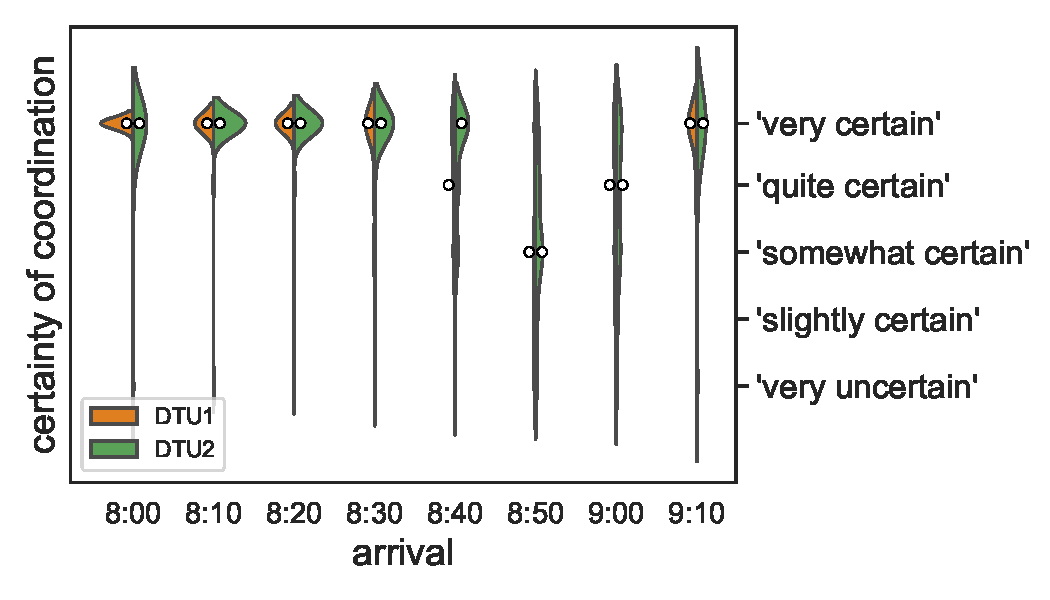
\includegraphics[width=0.8\linewidth]{tark_fig2_certainties}
\caption{Violin plots of certainty estimates. In each round, participants were asked how certain they were of successful coordination with their colleague. \modified{Orange areas show the results from DTU1 ($\text{n}=2160$) and green areas the results from DTU2 ($\text{n}=1012$).} We predefined a five point likert scale of certainty estimates as: `very uncertain', `slightly certain, `somewhat certain', `quite certain', and `very certain', and translated them into the numerical values of probability estimates used in the payoff calculations (see Appendix~\ref{appendix:payoffs}). The white dots correspond to the median certainty estimate.}
\label{fig:certain}
\end{figure}

The violin plots in Fig.~\ref{fig:certain} show the distribution of certainty estimates for each arrival time. In general, Fig.~\ref{fig:certain} shows that it is exceedingly rare for any of the participants to consider it problematic to go to the canteen when arriving early. Arriving at $8{:}30$ or earlier is deemed sufficiently early to visit the canteen with very high confidence. \modified{The DTU1 participants appear to be more aware of the danger of miscoordination than the DTU2 participants (mean certainty $0.73$ against $0.79$ at $8{:}50$), and they also choose the canteen less often at $8{:}50$ ($43\%$ against $64\%$, Fig.~\ref{fig:1}).} The differences between the experiments are however still relatively minor.

\begin{figure}[htb]
\centering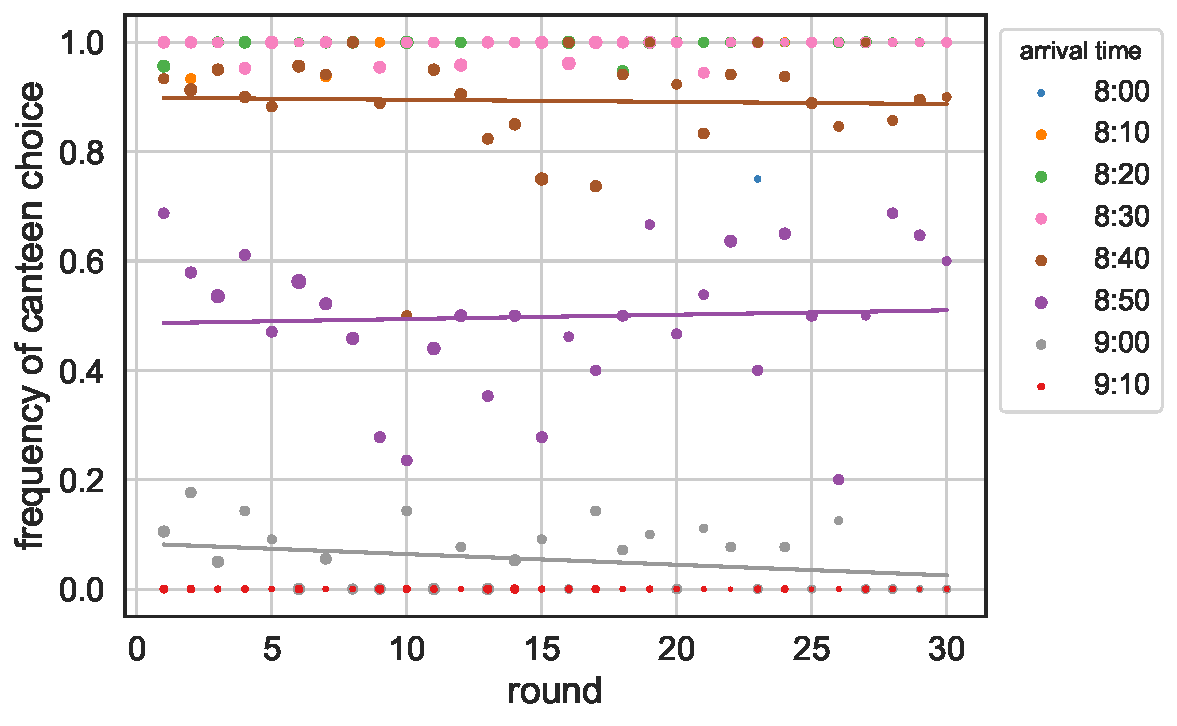
\includegraphics[width=0.8\linewidth]{tark_fig4_timeseries}
\caption{Mean frequencies of canteen choices for all possible arrival times as a function of the number of rounds played\modified{, DTU1 and DTU2 combined}. The three fitted horizontal lines, corresponding to arrival times $8{:}40$, $8{:}50$, and $9{:}00$ respectively, represent \modified{weighted least squares} (WLS) with the weights chosen to be the square root of the number of data points constituting the mean frequencies for each round, also shown by dot size.}
\label{timeseries}
\end{figure}
Fig.~\ref{timeseries} shows the mean frequency of canteen choices as a function of rounds played \modified{for the two DTU experiments}. Each color corresponds to a certain arrival time. Clearly, the only arrival times that do not converge towards either the canteen or the office are the arrival times of $8{:}40$ and $8{:}50$, with the former fluctuating around $90\%$ canteen choices and the latter fluctuating around $50\%$ canteen choices. This indicates that there is no behavioral change during the game. Participants arriving at $8{:}40$ or $8{:}50$ do not feel incentivized to change their behavior significantly in subsequent rounds, even though there is a high risk of miscoordination. This is not to say that participants do not learn that canteen choices at $8{:}40$ or $8{:}50$ are dangerous. Partitioning the data from Fig.~\ref{fig:1} into two bins, corresponding to pairs having had no miscoordination and pairs having had one or more miscoordinations (see the supplementary data analysis in Appendix~\ref{app:supplementary-data-analysis}), shows somewhat decreasing certainty estimates around the critical arrival times. However, this does not affect their actual choices. So even though participants learn that their choices are risky, they do not see any way to improve their strategy (at least not in the short term).

\begin{figure}[htb]
  \centering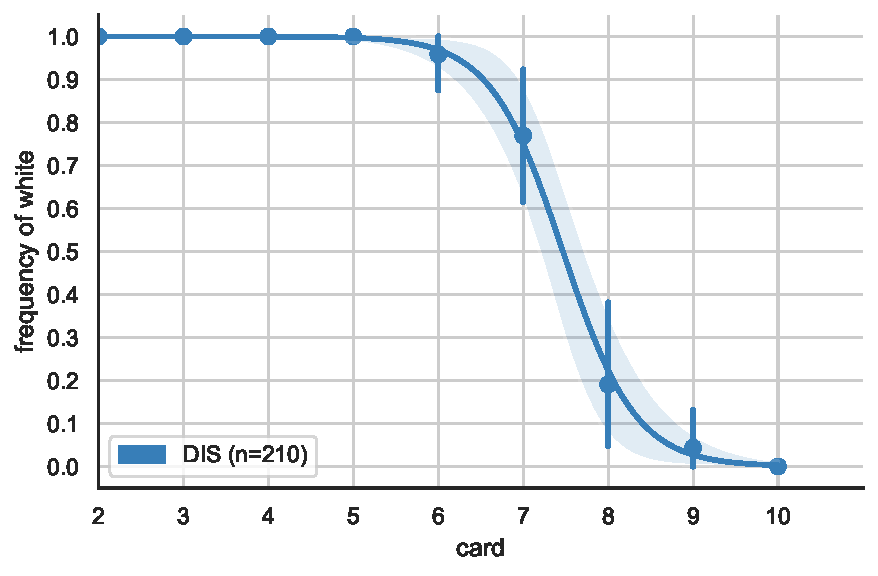
\includegraphics[width=0.6\linewidth]{tark_fig5_DIS}
  \caption{Logistic regression of the relationship between card number and choice of a white stone in the qualitative experiment at DIS. The resulting curve shows a very similar overall trend as in the main experiments shown in Fig.~\ref{fig:1}.} 
  \label{fig:dis} 
\end{figure}


%\subsection{Conflict of Interest}
%The authors declare no conflict of interest.



%\subsection{Author contributions} % \small 

%\subsection{Open Research badges}
%\tobo{Fix this. Probably a footnote somewhere.}
%This article has earned Open Data badge. Data is available at www.github.com/gavstrik/cd.

